\documentclass[12pt, twoside]{article}
\usepackage[letterpaper, margin=1in, headsep=0.5in]{geometry}
\usepackage[english]{babel}
\usepackage[utf8]{inputenc}
\usepackage{amsmath}
\usepackage{amsfonts}
\usepackage{amssymb}
\usepackage{tikz}
\usetikzlibrary{quotes, angles}
\usepackage{graphicx}
\usepackage{enumitem}
\usepackage{multicol}

\newif\ifmeta
\metatrue %print standards and topics tags

\title{Regents Geometry}
\author{Chris Huson}
\date{September 2020}

\usepackage{fancyhdr}
\pagestyle{fancy}
\fancyhf{}
\renewcommand{\headrulewidth}{0pt} % disable the underline of the header
\raggedbottom


\fancyhead[LE]{\thepage}
\fancyhead[RO]{\thepage \\ Name: \hspace{4cm} \,\\}
\fancyhead[LO]{BECA / Dr. Huson / Geometry 01-Intro\\* pset ID: 12}

\begin{document}

\subsubsection*{1-7Exam-Intro}
\begin{enumerate}
\item I have a calculator. (circle one). Yes \qquad No
\item I have a compass, ruler, protractor, notebook, and folder (circle one). Yes \qquad No
\vspace{0.5cm}
\item Complete the construction of an equilateral triangle and complete the six steps.
  \begin{enumerate}
    \item Given the line segment $\overline{MN}$.
    \bigskip
    \item Construct circle $M$ with radius $MN$.
    \bigskip
    \item Construct circle $\rule{2cm}{0.15mm}$  with radius $MN$. \bigskip
    \item Label the intersection $P$ of the two circles.
    \bigskip
    \item Draw line segment $\overline{MP}$ and line segment $\rule{2cm}{0.15mm}$
    \bigskip
    \item $\triangle MNP$ is equilateral.
  \end{enumerate}
  \vspace{7cm}
  \begin{center}
  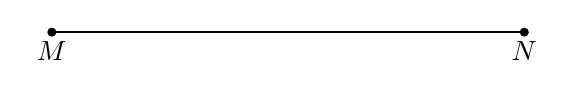
\begin{tikzpicture}
    \draw [-, thick] (0,0)--(6,0);
    \draw [fill] (0,0) circle [radius=0.05] node[below]{$M$};
    \draw [fill] (6,0) circle [radius=0.05] node[below]{$N$};
  \end{tikzpicture}
  \end{center}

\newpage
\item Points that are all located on the same plane are $\rule{4cm}{0.15mm}$.\bigskip

\item Draw and label a line segment $\overline{AB}$ such that the distance between points $A$ and $B$ is 4 cm. 
  \vspace{3cm}

\item Identify three points in the given plane.\\[0.25in]
    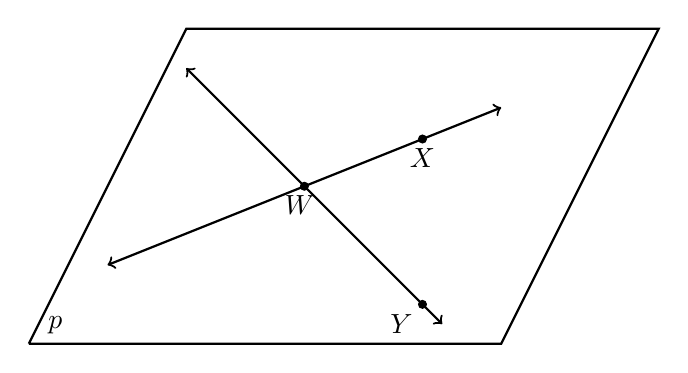
\begin{tikzpicture}
      \draw [thick](0,0) node[above right]{$\ p$} --(6,0)--(8,4)--(2,4)--(0,0);
      \draw [<->, thick] (1,1)--(6,3);
      \draw [fill] (3.5,2) circle [radius=0.05] node[below]{$W \ $};
      \draw [fill] (5,2.6) circle [radius=0.05] node[below]{$X$};
      \draw [<->, thick] (2,3.5)--(5.25,.25);
      \draw [fill] (5,0.5) circle [radius=0.05] node[below left]{$Y$};
    \end{tikzpicture} \vspace{1cm}

\item A flat surface is a(n) $\rule{4cm}{0.15mm}$. \bigskip
  
\item Two line segments or angles of equal measure are $\rule{4cm}{0.15mm}$. \bigskip

\item Given $\overline{DEF}$, $DE=5 \frac{1}{2}$, and $EF=2 \frac{1}{2}$.
  \begin{enumerate}
    \item Find ${DF}$.\\[.5in]
      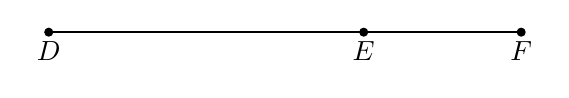
\begin{tikzpicture}
        \draw [-, thick] (1,0)--(7,0);
        \draw [fill] (1,0) circle [radius=0.05] node[below]{$D$};
        \draw [fill] (5,0) circle [radius=0.05] node[below]{$E$};
        \draw [fill] (7,0) circle [radius=0.05] node[below]{$F$};
      \end{tikzpicture} \vspace{2cm}
    \item The postulate used in this problem is the \rule{6cm}{0.15mm}.
  \end{enumerate}

\newpage
\item Given the points $V$ and $W$, draw $\overrightarrow{WV}$.\\
  \vspace{1cm}
  \begin{center}
    \begin{tikzpicture}
    \draw [fill] (0,2) circle [radius=0.05] node[below]{$V$};
    \draw [fill] (5,0) circle [radius=0.05] node[below]{$W$};
  \end{tikzpicture}
  \end{center}
  \vspace{1cm}

\item Use symbols to write the name of each geometric figure.\\.\\
    \vspace{0.5cm}
    \begin{tikzpicture}
      \draw [->, thick] (0,0)--(3,1.5);
      \draw [fill] (0,0) circle [radius=0.05] node[below]{$G$};
      \draw [fill] (2,1) circle [radius=0.05] node[below]{$H$};
      \node at (-1,0) {(a)};
    \end{tikzpicture}  \hspace{.1cm}
    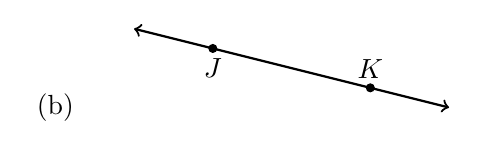
\begin{tikzpicture}
      \draw [<->, thick] (1,1)--(5,0);
      \draw [fill] (2,0.75) circle [radius=0.05] node[below]{$J$};
      \draw [fill] (4,.25) circle [radius=0.05] node[above]{$K$};
      \node at (0,0) {(b)};
    \end{tikzpicture} \hspace{.25cm}
    \begin{tikzpicture}
      \draw [-, thick] (1,0)--(4,2);
      \draw [fill] (1,0) circle [radius=0.05] node[below]{$L$};
      \draw [fill] (4,2) circle [radius=0.05] node[above left]{$M$};
      \node at (0,0) {(c)};
    \end{tikzpicture}
    \vspace{1cm}

\item Using a straightedge, draw a pair of opposite rays. Label any points in the drawing and name the two rays to the right of the drawing, using proper notation.\smallskip
  \vspace{3cm}

\item Given $\overleftrightarrow{PQ}$ as shown on the number line. \\[20pt] % Midpoint
  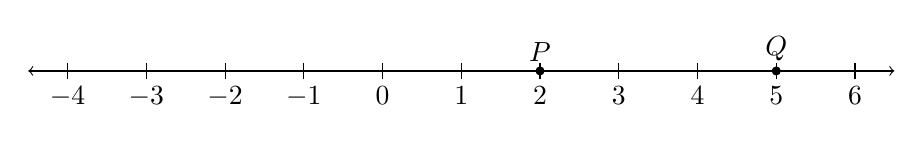
\begin{tikzpicture}
    \draw [<->] (-4.5,0)--(6.5,0);
    \foreach \x in {-4,...,6} %2 leading for diff!=1
      \draw[shift={(\x,0)},color=black] (0pt,-3pt) -- (0pt,3pt) node[below=5pt]  {$\x$};
      \draw [fill] (2,0) circle [radius=0.05] node[above] {$P$};
      \draw [fill] (5,0) circle [radius=0.05] node[above] {$Q$};
  \end{tikzpicture} \\ \bigskip
  What is the distance on the number line between the points $P$ and $Q$? \vspace{2cm}  

\newpage
\item Given $\triangle ABC$ with $\overline{AB} \cong \overline{AC}$. On the diagram mark the congruent line segments with tick marks.
  \begin{center}
  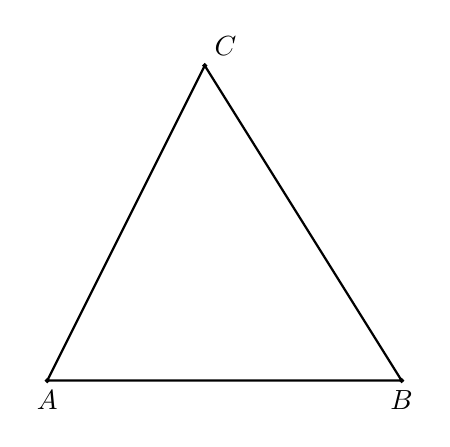
\begin{tikzpicture}[scale=0.5]
    \draw [thick](0,0)--(9,0)--(4,8)--(0,0);
    \draw [fill] (0,0) circle [radius=0.05] node[below]{$A$};
    \draw [fill] (9,0) circle [radius=0.05] node[below]{$B$};
    \draw [fill] (4,8) circle [radius=0.05] node[above right]{$C$};
  \end{tikzpicture}
  \end{center}
  \vspace{1cm}

\item Find the measure of the angle in degrees and the given segment's length in centimeters. \vspace{0.25cm}
  \begin{enumerate}
    \item  $m \angle GEF = $ \rule{4cm}{0.15mm} \bigskip
    \item  $EG=$ \rule{4cm}{0.15mm} \bigskip
    \item Name a pair of opposite rays: \rule{4cm}{0.15mm} \bigskip
  \end{enumerate}
  \begin{center}
  \begin{tikzpicture}[scale=1.5]
    \draw [->, thick] (0,0)--(35:5);
    \draw [<->, thick] (-3,0)--(7,0);
    %\draw [->, thick] (0,0)--(-1.2,3);
    %\draw [fill] (-1,2.5) circle [radius=0.05] node[left ]{$B$};
    \draw [fill] (35:3) circle [radius=0.05] node[above left ]{$G$};
    \draw [fill] (-2,0) circle [radius=0.05] node[below]{$D$};
    \draw [fill] (0,0) circle [radius=0.05] node[below]{$E$};
    \draw [fill] (4,0) circle [radius=0.05] node[above]{$F$};
  \end{tikzpicture}
  \end{center}

\newpage
\item Given $\overline{ABC}$, $AB=3x-4$, $BC=x+5$, $AC=13$. Find ${BC}$. \\ 
    Check your answer for full credit.
    \vspace{1cm}
      \begin{center}
        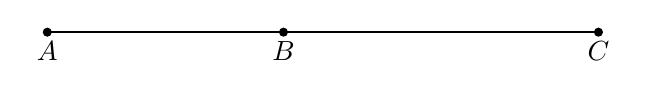
\begin{tikzpicture}
            \draw [-, thick] (0,0)--(7,0);
            \draw [fill] (0,0) circle [radius=0.05] node[below]{$A$};
            \draw [fill] (3,0) circle [radius=0.05] node[below]{$B$};
            \draw [fill] (7,0) circle [radius=0.05] node[below]{$C$};
        \end{tikzpicture}
      \end{center} \vspace{7cm}

\item Given the rectangle $ABCD$ shown below.
  \begin{enumerate}
    \item Measure and mark the length and width of the rectangle in centimeters.
    \item Calculate the area of the rectangle in square centimeters. (show your work)
  \end{enumerate}
  \vspace{1cm}
  \begin{center}
  \begin{tikzpicture}
    \draw [-, thick] (0,0)--(7,0)--(7,4)--(0,4)--cycle;
    \draw [fill] (0,0) circle [radius=0.05] node[left]{$A$};
    \draw [fill] (7,0) circle [radius=0.05] node[right]{$B$};
    \draw [fill] (7,4) circle [radius=0.05] node[right]{$C$};
    \draw [fill] (0,4) circle [radius=0.05] node[left]{$D$};
  \end{tikzpicture}
  \end{center}

\newpage
\item Use each term according to its geometric meaning: ``sketch", ``draw", ``construct".
  \begin{enumerate}
    \item $\rule{4cm}{0.15mm}$ is to make a freehand diagram showing important features. \smallskip
    \item $\rule{4cm}{0.15mm}$ is to depict with accurate measures using ruler, protractor, and compass. \smallskip
    \item $\rule{4cm}{0.15mm}$ is a formal, logical process to create geometric figures using only a straightedge and compass.
  \end{enumerate} \smallskip

\item Given the situation in the diagram, answer each question. Circle True or False. 
  \vspace{0.25cm}
      \begin{flushright}
      \begin{tikzpicture}[scale=1]
        \draw [->, thick] (0,0)--(50:5);
        \draw [<->, thick] (-5,.5)--(5,-.5);
        \draw [->, thick] (0,0)--(-1.2,3);
        \draw [fill] (-1,2.5) circle [radius=0.05] node[left ]{$S$};
        \draw [fill] (50:3) circle [radius=0.05] node[above left ]{$T$};
        \draw [fill] (0,0) circle [radius=0.05] node[below]{$P$};
        \draw [fill] (4,-0.4) circle [radius=0.05] node[above]{$U$};
        \draw [fill] (-4,0.4) circle [radius=0.05] node[above]{$R$};
      \end{tikzpicture}
      \end{flushright}
    \begin{enumerate}
      \item True or False: $\overrightarrow{PR}$ and $\overrightarrow{PU}$ are opposite rays.\bigskip
      \item True or False: $\angle TPR$ is an obtuse angle.\bigskip
      \item True or False: $\angle RPS$ and $\angle TPU$ are adjacent angles. \bigskip
    \end{enumerate}

\item In the following two problems, solve for the value of $x$.
  \begin{multicols}{2}
    \begin{enumerate}
      \item   $3(x-5)=-33$ \vspace{6cm}
      \item   $3-\frac{1}{2} x=2$ \vspace{6cm}
    \end{enumerate}
  \end{multicols}
    \vspace{3cm}

\end{enumerate}
\end{document}